
\section{System Model}

% ˫����ʽ�м��������ͼ��:��\begin{figure}�м���*���ɣ�����\begin{figure*}  \end{figure*} ��

\begin{figure}[htb]
  \centering
 %\setlength{\abovecaptionskip}{-15pt}
 %\setlength{\belowcaptionskip}{-5pt}
    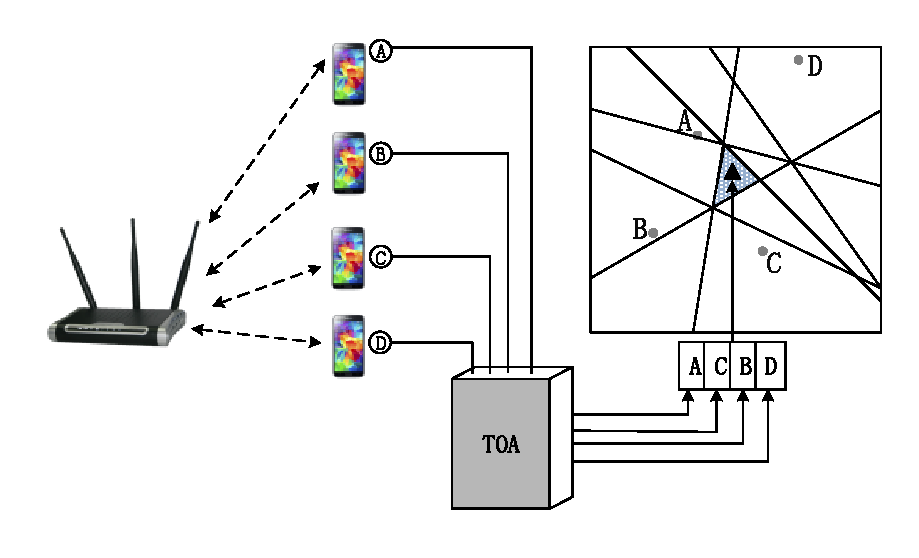
\includegraphics[height=4.5cm]{image/fig1.pdf} 
    \caption{Overview of HPI-SBL}
 \label{overview}
    \end{figure}


In this section, we focus mainly on the system overview of our HPI-SBL system, which aims at locating an acoustic source with the node sequence. 
Fig.1 shows a layout of a acoustic sensor network with $N$ sensor nodes and the acoustic source.
We use circles and the triangle to stand for sensor nodes and the acoustic source, respectively.
Consider any two reference nodes and draw a perpendicular bisector to the line joining their locations. This perpendicular bisector divides the localization
space into two different regions that are distinguished by their proximity to either reference nodes, as illustrated in Fig.1. 
Similarly, if perpendicular bisectors are drawn for all pairs of reference nodes, they can divide the localization space into many regions.
All locations inside a region have the same node sequence, and the node sequence of a given region is unique to that region.
If each region in the arrangement is represented by its centroid, then there exists a one-to-one mapping between a node sequence and the centroid of the region that it represents.

Briefly, sequence-based localization system works as follows. 
Sensor nodes detect the acoustic event sequentially at different time instances, then an order of related nodes, called node sequence, is naturally generated. 
For instance, in Fig.1, when the acoustic source generates a wave, the node sequence $NodeSeq (A C B D)$ is obtained along the sound propagation. 
The node sequence implies the location information of the acoustic source. 
By gathering the TOA measurement data from sensor nodes, the location of the acoustic source can be estimated by processing the node sequence. 

Fig.2 shows that $NodeSeq (A C B D)$ can be achieved by TOA measurement of the acoustic event.
We can get the distance sequence ${SA} < {SC} < {SB} < {SD}$ from each node to the acoustic source $S$.
$SA<SC$ shows that the acoustic source $S$ lies in the right half-plane of the perpendicular bisector of A and C.
Similarly, $SC<SB$ means that the acoustic source $S$ lies in the left half-plane of the perpendicular bisector of C and B.
$SB<SD$ shows that the acoustic source $S$ lies in the left half-plane of the perpendicular bisector of B and D.
The intersection of the three half-planes is the final region of the acoustic source.


    \begin{figure}[!htb]
    \centering
 \setlength{\abovecaptionskip}{-15pt}
                     \vspace{-3.5mm}  
 %\setlength{\belowcaptionskip}{-5pt}
    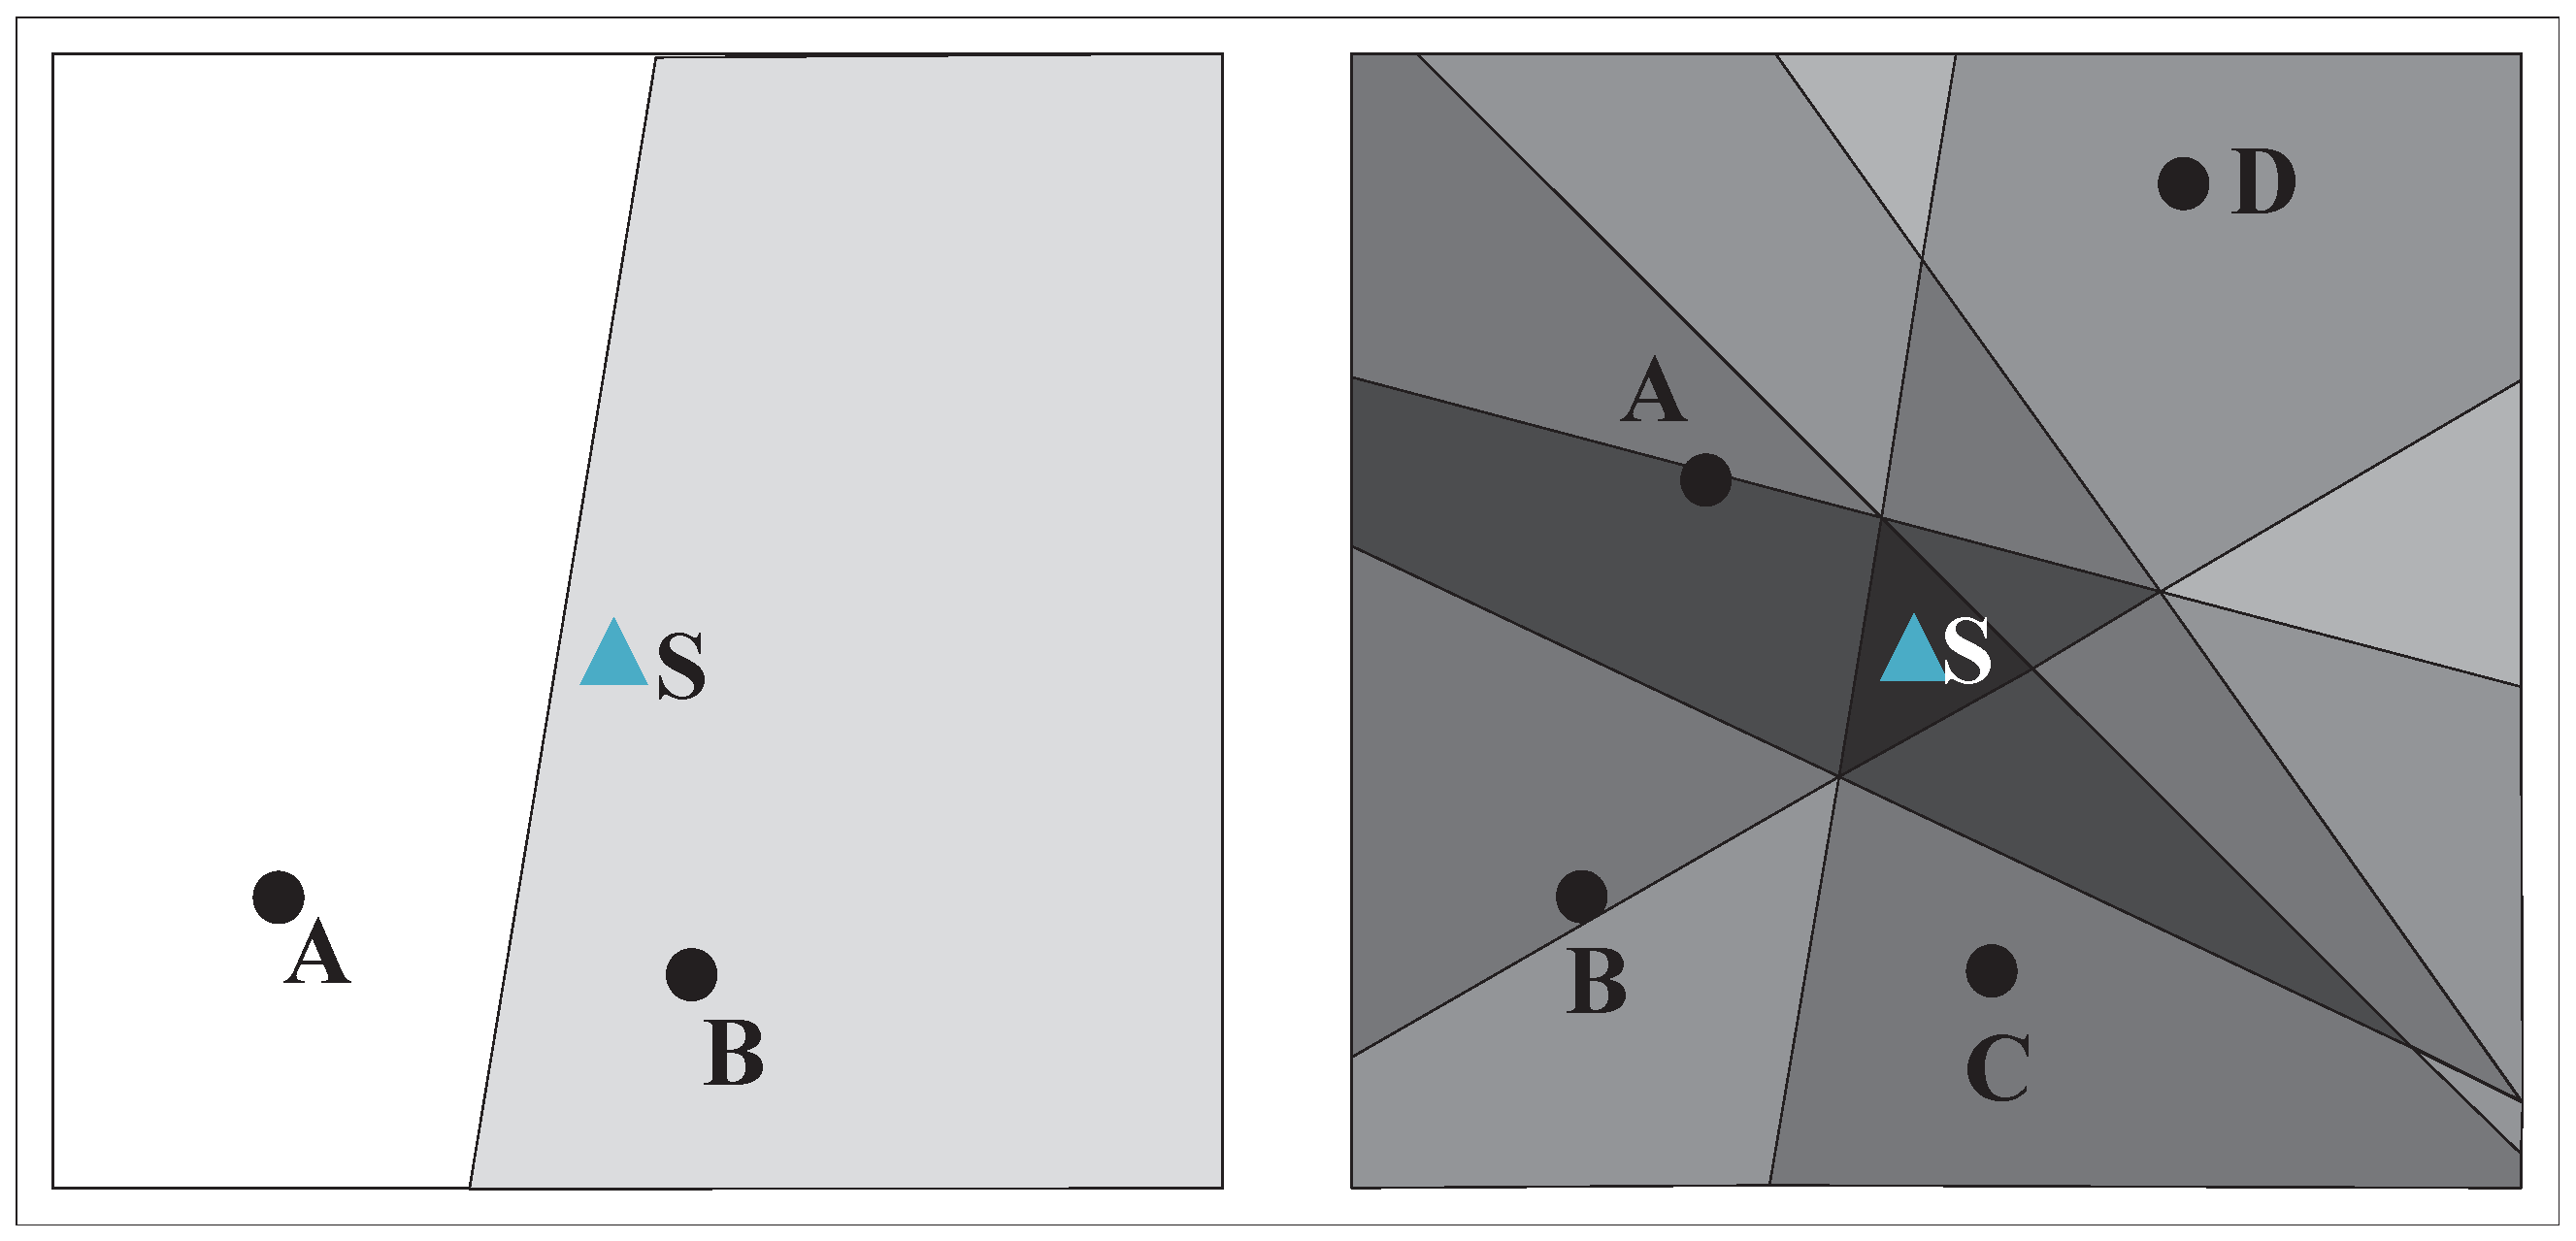
\includegraphics[height=4cm]{image/fig2.eps} 
	\vspace{10mm}
    \caption{The basic idea of HPI-SBL}
	\label{fig2}
    \vspace{-3.5mm}
    \end{figure}

	
Compared to earlier works on sequence-based localization  with brute force searching scheme (SBL~\cite{yedavalli2008sequence}), 
we carefully formulate sequence-based localization as the traditional half-plane intersection problem. 
To the best of our knowledge, this is the first work to leverage half-plane intersection for solving sequence-based localization problems in sensor networks.





